\documentclass{beamer}
\usepackage[utf8]{inputenc}

\usetheme{Madrid}
\usecolortheme{default}
\usepackage{amsmath,amssymb,amsfonts,amsthm}
\usepackage{txfonts}
\usepackage{tkz-euclide}
\usepackage{listings}
\usepackage{adjustbox}
\usepackage{array}
\usepackage{tabularx}
\usepackage{gvv} 
\usepackage{lmodern}
\usepackage{circuitikz}
\usepackage{tikz}
\usepackage{graphicx}
\usepackage{comment}

\setbeamertemplate{page number in head/foot}[totalframenumber]

\usepackage{tcolorbox}
\tcbuselibrary{minted,breakable,xparse,skins}

\definecolor{bg}{gray}{0.95}
\DeclareTCBListing{mintedbox}{O{}m!O{}}{%
breakable=true,
listing engine=minted,
listing only,
minted language=#2,
minted style=default,
minted options={%
linenos,
gobble=0,
breaklines=true,
breakafter=,,
fontsize=\small,
numbersep=8pt,
#1},
boxsep=0pt,
left skip=0pt,
right skip=0pt,
left=25pt,
right=0pt,
top=3pt,
bottom=3pt,
arc=5pt,
leftrule=0pt,
rightrule=0pt,
bottomrule=2pt,
toprule=2pt,
colback=bg,
colframe=orange!70,
enhanced,
overlay={%
\begin{tcbclipinterior}
\fill[orange!20!white] (frame.south west) rectangle ([xshift=20pt]frame.north west);
\end{tcbclipinterior}},
#3,
}
\lstset{
language=C,
basicstyle=\ttfamily\small,
keywordstyle=\color{blue},
stringstyle=\color{orange},
commentstyle=\color{green!60!black},
numbers=left,
numberstyle=\tiny\color{gray},
breaklines=true,
showstringspaces=false,
}

\title
{2.10.71}
\date{September 27, 2025}
\author
{EE25BTECH11043 - Nishid Khandagre}

\begin{document}

\frame{\titlepage}

\begin{frame}{Question}
If the vectors $\vec{b}$, $\vec{c}$, $\vec{d}$ are not coplanar, then prove that the vector
$\myvec{\vec{a} \times\vec{b}} \times\myvec{\vec{c} \times\vec{d}} + \myvec{\vec{a} \times\vec{c}} \times\myvec{\vec{d} \times\vec{b}} + \myvec{\vec{a} \times\vec{d}} \times\myvec{\vec{b} \times\vec{c}}$
is parallel to $\vec{a}$.
\end{frame}

\begin{frame}{Theoretical Solution}
The vector triple product $\vec{A} \times \myvec{\vec{B} \times \vec{C}}$ can be written as:
\begin{align}
\vec{A} \times \myvec{\vec{B} \times \vec{C}} &= \vec{B}\myvec{\vec{A}^\top \vec{C}} - \vec{C}\myvec{\vec{A}^\top \vec{B}}
\end{align}
Also, we know
\begin{align}
\myvec{\vec{A} \times \vec{B}} \times \vec{C} = - \vec{C} \times \myvec{\vec{A} \times \vec{B}}
\end{align}
\end{frame}

\begin{frame}{Theoretical Solution}
\begin{align}
\myvec{\vec{A} \times \vec{B}} \times \myvec{\vec{C} \times \vec{D}} = \myvec{\vec{A}^\top \myvec{\vec{C} \times \vec{D}}} \vec{B} - \myvec{\vec{B}^\top \myvec{\vec{C} \times \vec{D}}} \vec{A}
\label{eq:equation}
\end{align}
By using \eqref{eq:equation}
\begin{align}
\myvec{\vec{a} \times\vec{b}}\times \myvec{\vec{c} \times\vec{d}}&= \myvec{\vec{a}^\top \myvec{\vec{c} \times \vec{d}}} \vec{b} - \myvec{\vec{b}^\top \myvec{\vec{c} \times \vec{d}}} \vec{a}\\
&=\sbrak{\vec{a} \ \vec{c} \ \vec{d}}\vec{b} - \sbrak{\vec{b} \ \vec{c} \ \vec{d}}\vec{a}
\end{align}
\end{frame}

\begin{frame}{Theoretical Solution}

\begin{align}
\myvec{\vec{a} \times\vec{c}} \times\myvec{\vec{d} \times\vec{b}}&=
\myvec{\vec{a}^\top \myvec{\vec{d} \times \vec{b}}} \vec{c} - \myvec{\vec{c}^\top \myvec{\vec{d} \times \vec{b}}} \vec{a}\\
&= \sbrak{\vec{a} \ \vec{d} \ \vec{b}}\vec{c} - \sbrak{\vec{c} \ \vec{d} \ \vec{b}}\vec{a} \\
&= -\sbrak{\vec{a} \ \vec{b} \ \vec{d}}\vec{c} + \sbrak{\vec{b} \ \vec{c} \ \vec{d}}\vec{a}
\end{align}
\end{frame}

\begin{frame}{Theoretical Solution}

\begin{align}
\myvec{\vec{a} \times\vec{d}} \times\myvec{\vec{b} \times\vec{c}}&=
\myvec{\vec{a}^\top \myvec{\vec{b} \times \vec{c}}} \vec{d} - \myvec{\vec{d}^\top \myvec{\vec{b} \times \vec{c}}} \vec{a}\\
&=\sbrak{\vec{a} \ \vec{b} \ \vec{c}}\vec{d} - \sbrak{\vec{d} \ \vec{b} \ \vec{c}}\vec{a} \\
&= \sbrak{\vec{a} \ \vec{b} \ \vec{c}}\vec{d} - \sbrak{\vec{b} \ \vec{c} \ \vec{d}}\vec{a}
\end{align}
\end{frame}

\begin{frame}{Theoretical Solution}
On adding :
\begin{align}
& \myvec{\vec{a} \times\vec{b}} \times\myvec{\vec{c} \times\vec{d}} + \myvec{\vec{a} \times\vec{c}} \times\myvec{\vec{d} \times\vec{b}} + \myvec{\vec{a} \times\vec{d}} \times\myvec{\vec{b} \times\vec{c}}\\
&= \sbrak{\vec{a} \ \vec{c} \ \vec{d}}\vec{b}-\sbrak{\vec{b} \ \vec{c} \ \vec{d}}\vec{a}-\sbrak{\vec{a} \ \vec{b} \ \vec{d}}\vec{c}+\sbrak{\vec{b} \ \vec{c} \ \vec{d}}\vec{a}+\sbrak{\vec{a} \ \vec{b} \ \vec{c}}\vec{d}-\sbrak{\vec{b} \ \vec{c} \ \vec{d}}\vec{a}\\
&= \sbrak{\vec{a} \ \vec{c} \ \vec{d}}\vec{b} - \sbrak{\vec{a} \ \vec{b} \ \vec{d}}\vec{c} + \sbrak{\vec{a} \ \vec{b} \ \vec{c}}\vec{d} - \sbrak{\vec{b} \ \vec{c} \ \vec{d}}\vec{a}
\end{align}
\end{frame}

\begin{frame}{Theoretical Solution}
Using the expansion of a vector $\vec{a}$ in terms of non-coplanar vectors $\vec{b}, \vec{c}, \vec{d}$:
\begin{align}
\vec{a}\sbrak{\vec{b} \ \vec{c} \ \vec{d}} = \sbrak{\vec{a} \ \vec{c} \ \vec{d}}\vec{b} + \sbrak{\vec{a} \ \vec{d} \ \vec{b}}\vec{c} + \sbrak{\vec{a} \ \vec{b} \ \vec{c}}\vec{d}
\end{align}
Rearranging the scalar triple products on the right:
\begin{align}
\vec{a}\sbrak{\vec{b} \ \vec{c} \ \vec{d}} = \sbrak{\vec{a} \ \vec{c} \ \vec{d}}\vec{b} - \sbrak{\vec{a} \ \vec{b} \ \vec{d}}\vec{c} + \sbrak{\vec{a} \ \vec{b} \ \vec{c}}\vec{d}
\end{align}
\end{frame}

\begin{frame}{Theoretical Solution}
Substitute this into the sum:
\begin{align}
&= \vec{a}\sbrak{\vec{b} \ \vec{c} \ \vec{d}} - \sbrak{\vec{b} \ \vec{c} \ \vec{d}}\vec{a} \\
&= \sbrak{\vec{b} \ \vec{c} \ \vec{d}}\vec{a} - \sbrak{\vec{b} \ \vec{c} \ \vec{d}}\vec{a} \\
&= \vec{0}
\end{align}
The resultant vector is $\vec{0}$.
A zero vector is considered parallel to any vector.
Thus, the given vector expression is parallel to $\vec{a}$.
\end{frame}

\begin{frame}[fragile]
\frametitle{C Code}
\begin{lstlisting}
#include <stdio.h>
#include <math.h>

// Function to calculate the cross product of two 3D vectors.
void cross_product(double ax, double ay, double az,
                    double bx, double by, double bz,
                    double *rx, double *ry, double *rz) {
    *rx = ay * bz - az * by;
    *ry = az * bx - ax * bz;
    *rz = ax * by - ay * bx;
}
\end{lstlisting}
\end{frame}

\begin{frame}[fragile]
\frametitle{C Code}
\begin{lstlisting}
// Function to calculate the dot product of two 3D vectors.
double dot_product(double ax, double ay, double az,
                    double bx, double by, double bz) {
    return ax * bx + ay * by + az * bz;
}
// Helper function to calculate a term of the form (V1 x V2) x (V3 x V4).
void calculate_vector_quad_cross(
    double v1x, double v1y, double v1z,
    double v2x, double v2y, double v2z,
    double v3x, double v3y, double v3z,
    double v4x, double v4y, double v4z,
    double *term_rx, double *term_ry, double *term_rz) {
\end{lstlisting}
\end{frame}

\begin{frame}[fragile]
\frametitle{C Code}
\begin{lstlisting}
// Helper function to calculate a term of the form (V1 x V2) x (V3 x V4).
void calculate_vector_quad_cross(
    double v1x, double v1y, double v1z,
    double v2x, double v2y, double v2z,
    double v3x, double v3y, double v3z,
    double v4x, double v4y, double v4z,
    double *term_rx, double *term_ry, double *term_rz) {

    // Calculate V1 x V2
    double v1xv2_x, v1xv2_y, v1xv2_z;
    cross_product(v1x, v1y, v1z, v2x, v2y, v2z, &v1xv2_x, &v1xv2_y, &v1xv2_z);
    \end{lstlisting}
\end{frame}

\begin{frame}[fragile]
\frametitle{C Code}
\begin{lstlisting}

    // Calculate V3 x V4
    double v3xv4_x, v3xv4_y, v3xv4_z;
    
    cross_product(v3x, v3y, v3z, v4x, v4y, v4z, &v3xv4_x, &v3xv4_y, &v3xv4_z);

    // Calculate (V1 x V2) x (V3 x V4)
    cross_product(v1xv2_x, v1xv2_y, v1xv2_z, v3xv4_x, v3xv4_y, v3xv4_z,
    term_rx, term_ry, term_rz);
\end{lstlisting}
\end{frame}

\begin{frame}[fragile]
\frametitle{C Code}
\begin{lstlisting}
// Main function to calculate the full expression:
// (a × b) × (c × d) + (a × c) × (d × b) + (a × d) × (b × c)
void calculate_full_expression(
    double ax, double ay, double az,
    double bx, double by, double bz,
    double cx, double cy, double cz,
    double dx, double dy, double dz,
    double *result_x, double *result_y, double *result_z) {

    double term1_x, term1_y, term1_z;
    double term2_x, term2_y, term2_z;
    double term3_x, term3_y, term3_z;

\end{lstlisting}
\end{frame}

\begin{frame}[fragile]
\frametitle{C Code}
\begin{lstlisting}
    // Term 1: (a x b) x (c x d)
    calculate_vector_quad_cross(ax, ay, az, bx, by, bz,
                                cx, cy, cz, dx, dy, dz,
                                &term1_x, &term1_y, &term1_z);

    // Term 2: (a x c) x (d x b)
    calculate_vector_quad_cross(ax, ay, az, cx, cy, cz,
                                dx, dy, dz, bx, by, bz,
                                &term2_x, &term2_y, &term2_z);
\end{lstlisting}
\end{frame}

\begin{frame}[fragile]
\frametitle{C Code}
\begin{lstlisting}
    // Term 3: (a x d) x (b x c)
    calculate_vector_quad_cross(ax, ay, az, dx, dy, dz,
                                bx, by, bz, cx, cy, cz,
                                &term3_x, &term3_y, &term3_z);

    // Sum the terms
    *result_x = term1_x + term2_x + term3_x;
    *result_y = term1_y + term2_y + term3_y;
    *result_z = term1_z + term2_z + term3_z;
}
\end{lstlisting}
\end{frame}

\begin{frame}[fragile]
\frametitle{C Code}
\begin{lstlisting}
// Function to check if three vectors are coplanar (scalar triple product is zero).
double scalar_triple_product(double bx, double by, double bz,
                             double cx, double cy, double cz,
                             double dx, double dy, double dz) {
    double cxd_x, cxd_y, cxd_z;
    cross_product(cx, cy, cz, dx, dy, dz, &cxd_x, &cxd_y, &cxd_z);
    return dot_product(bx, by, bz, cxd_x, cxd_y, cxd_z);
}
\end{lstlisting}
\end{frame}

\begin{frame}[fragile]
\frametitle{Python Code (using C shared library)}
\begin{lstlisting}
import ctypes
import numpy as np
import matplotlib.pyplot as plt
from mpl_toolkits.mplot3d import Axes3D

# Load the shared library
lib_vector = ctypes.CDLL("./code5.so")

# Define argument types and return types for C functions
lib_vector.cross_product.argtypes = [
    ctypes.c_double, ctypes.c_double, ctypes.c_double,
    ctypes.c_double, ctypes.c_double, ctypes.c_double,
    ctypes.POINTER(ctypes.c_double), ctypes.POINTER(ctypes.c_double), ctypes.POINTER(ctypes.c_double)
]
\end{lstlisting}
\end{frame}

\begin{frame}[fragile]
\frametitle{Python Code (using C shared library)}
\begin{lstlisting}
lib_vector.cross_product.restype = None

lib_vector.dot_product.argtypes = [
    ctypes.c_double, ctypes.c_double, ctypes.c_double,
    ctypes.c_double, ctypes.c_double, ctypes.c_double
]
lib_vector.dot_product.restype = ctypes.c_double

lib_vector.calculate_vector_quad_cross.argtypes = [
    ctypes.c_double, ctypes.c_double, ctypes.c_double,
    ctypes.c_double, ctypes.c_double, ctypes.c_double,
    ctypes.c_double, ctypes.c_double, ctypes.c_double,
    ctypes.c_double, ctypes.c_double, ctypes.c_double,
    ctypes.POINTER(ctypes.c_double), ctypes.POINTER(ctypes.c_double), ctypes.POINTER(ctypes.c_double)
]
\end{lstlisting}
\end{frame}

\begin{frame}[fragile]
\frametitle{Python Code (using C shared library)}
\begin{lstlisting}
lib_vector.calculate_vector_quad_cross.restype = None

lib_vector.calculate_full_expression.argtypes = [
    ctypes.c_double, ctypes.c_double, ctypes.c_double,
    ctypes.c_double, ctypes.c_double, ctypes.c_double,
    ctypes.c_double, ctypes.c_double, ctypes.c_double,
    ctypes.c_double, ctypes.c_double, ctypes.c_double,
    ctypes.POINTER(ctypes.c_double), ctypes.POINTER(ctypes.c_double), ctypes.POINTER(ctypes.c_double)
]
lib_vector.calculate_full_expression.restype = None

\end{lstlisting}
\end{frame}

\begin{frame}[fragile]
\frametitle{Python Code (using C shared library)}
\begin{lstlisting}
lib_vector.scalar_triple_product.argtypes = [
    ctypes.c_double, ctypes.c_double, ctypes.c_double,
    ctypes.c_double, ctypes.c_double, ctypes.c_double,
    ctypes.c_double, ctypes.c_double, ctypes.c_double
]
lib_vector.scalar_triple_product.restype = ctypes.c_double

# Define arbitrary non-coplanar vectors b, c, d
b_np = np.array([1.0, 0.0, 0.0])
c_np = np.array([0.0, 1.0, 0.0])
d_np = np.array([0.0, 0.0, 1.0])

# Test coplanarity
stp_val = lib_vector.scalar_triple_product(
    b_np[0], b_np[1], b_np[2], c_np[0], c_np[1], c_np[2], d_np[0], d_np[1], d_np[2]
)
\end{lstlisting}
\end{frame}

\begin{frame}[fragile]
\frametitle{Python Code (using C shared library)}
\begin{lstlisting}
print(f"Scalar Triple Product of b, c, d: {stp_val}")
if np.isclose(stp_val, 0.0):
    print("Warning: Vectors b, c, d might be coplanar. Please choose different vectors.")
else:
    print("Vectors b, c, d are not coplanar (as required).")

# Define an arbitrary vector a
a_np = np.array([2.0, 3.0, 4.0])

# Ctypes doubles to hold the result
result_x = ctypes.c_double()
result_y = ctypes.c_double()
result_z = ctypes.c_double()
\end{lstlisting}
\end{frame}

\begin{frame}[fragile]
\frametitle{Python Code (using C shared library)}
\begin{lstlisting}
# Call the C function to calculate the full expression
lib_vector.calculate_full_expression(
    a_np[0], a_np[1], a_np[2], b_np[0], b_np[1], b_np[2],
    c_np[0], c_np[1], c_np[2], d_np[0], d_np[1], d_np[2],
    ctypes.byref(result_x), ctypes.byref(result_y), ctypes.byref(result_z)
)

calculated_vector_np = np.array([result_x.value, result_y.value, result_z.value])

print(f"\nVector a: {a_np}")
print(f"Calculated expression vector: {calculated_vector_np}")

is_parallel = False
    \end{lstlisting}
\end{frame}

\begin{frame}[fragile]
\frametitle{Python Code (using C shared library)}
\begin{lstlisting}
if np.allclose(calculated_vector_np, np.array([0,0,0])):
    is_parallel = True
elif np.allclose(a_np, np.array([0,0,0])):
    is_parallel = True
else:
    cross_prod_check = np.cross(a_np, calculated_vector_np)
    if np.allclose(cross_prod_check, np.array([0, 0, 0])):
        is_parallel = True
        if np.linalg.norm(a_np) > 1e-9:
            k = np.dot(calculated_vector_np, a_np) / np.dot(a_np, a_np)
            print(f"Scalar multiple k: {k:.4f}")
            print(f"Check: k * a = {k * a_np}")
\end{lstlisting}
\end{frame}

\begin{frame}[fragile]
\frametitle{Python Code (using C shared library)}
\begin{lstlisting}
if is_parallel:
    print("\nResult: The calculated vector is parallel to vector 'a'.")
else:
    print("\nResult: The calculated vector is NOT parallel to vector 'a'.")
# --- Plotting the vectors in 3D ---
fig = plt.figure(figsize=(10, 8))
ax = fig.add_subplot(111, projection='3d')
origin = [0, 0, 0]

ax.quiver(*origin, a_np[0], a_np[1], a_np[2], color='blue', arrow_length_ratio=0.1, label='Vector a')
ax.text(a_np[0], a_np[1], a_np[2], 'a', color='blue')
\end{lstlisting}
\end{frame}

\begin{frame}[fragile]
\frametitle{Python Code (using C shared library)}
\begin{lstlisting}
ax.quiver(*origin, b_np[0], b_np[1], b_np[2], color='red', arrow_length_ratio=0.2, label='Vector b')
ax.text(b_np[0], b_np[1], b_np[2], 'b', color='red')
ax.quiver(*origin, c_np[0], c_np[1], c_np[2], color='green', arrow_length_ratio=0.2, label='Vector c')
ax.text(c_np[0], c_np[1], c_np[2], 'c', color='green')

ax.quiver(*origin, d_np[0], d_np[1], d_np[2], color='purple', arrow_length_ratio=0.2, label='Vector d')
ax.text(d_np[0], d_np[1], d_np[2], 'd', color='purple')
scale_factor = 0.5
calculated_vector_scaled = calculated_vector_np * scale_factor
\end{lstlisting}
\end{frame}

\begin{frame}[fragile]
\frametitle{Python Code (using C shared library)}
\begin{lstlisting}
ax.quiver(*origin,
          calculated_vector_scaled[0], calculated_vector_scaled[1], calculated_vector_scaled[2],
          color='black', arrow_length_ratio=0.05, label='Resultant Vector (scaled)')
ax.set_xlim([-5, 5])
ax.set_ylim([-5, 5])
ax.set_zlim([-5, 5])
ax.set_xlabel('X-axis')
ax.set_ylabel('Y-axis')
ax.set_zlabel('Z-axis')
ax.legend()
plt.grid(True)
plt.savefig("fig1.png")
plt.show()
\end{lstlisting}
\end{frame}

\begin{frame}[fragile]
\frametitle{Python Code: Direct}
\begin{lstlisting}
import numpy as np
import matplotlib.pyplot as plt
from mpl_toolkits.mplot3d import Axes3D

def vector_triple_product_expansion(A, B, C):
    """
    Calculates the vector triple product A x (B x C) using the identity:
    A x (B x C) = (A . C) B - (A . B) C
    """
    return np.dot(A, C) * B - np.dot(A, B) * C
\end{lstlisting}
\end{frame}

\begin{frame}[fragile]
\frametitle{Python Code: Direct}
\begin{lstlisting}
def prove_parallel_to_a(a, b, c, d):
    """
    Proves that (a x b) x (c x d) + (a x c) x (d x b) + (a x d) x (b x c)
    is parallel to a, given that b, c, d are not coplanar.
    """
    # Term 1: (a x b) x (c x d)
    term1 = np.dot(np.cross(a, b), d) * c - np.dot(np.cross(a, b), c) * d
    # Term 2: (a x c) x (d x b)
    term2 = np.dot(np.cross(a, c), b) * d - np.dot(np.cross(a, c), d) * b

    # Term 3: (a x d) x (b x c)
    term3 = np.dot(np.cross(a, d), c) * b - np.dot(np.cross(a, d), b) * c
\end{lstlisting}
\end{frame}

\begin{frame}[fragile]
\frametitle{Python Code: Direct}
\begin{lstlisting}
    # Sum of the three terms
    result_vector = term1 + term2 + term3

    return result_vector

# --- Example Usage and Visualization ---
# Define non-coplanar vectors b, c, d
b = np.array([1, 0, 0])
c = np.array([0, 1, 0])
d = np.array([0, 0, 1])

# Define vector a
a = np.array([2, 3, 4])
# Prove the identity
result_vector = prove_parallel_to_a(a, b, c, d)
\end{lstlisting}
\end{frame}

\begin{frame}[fragile]
\frametitle{Python Code: Direct}
\begin{lstlisting}
# Check if result_vector is parallel to a
cross_product_check = np.cross(result_vector, a)

print(f"Vector a: {a}")
print(f"Resulting vector: {result_vector}")
print(f"Cross product of result_vector and a (should be close to zero for parallel): {cross_product_check}")

# Calculate a scalar multiple to show parallelism
scalar_multiple = np.dot(b, np.cross(c, d))
expected_result = scalar_multiple * a

print(f"Expected result based on identity [b c d] * a: {expected_result}")
\end{lstlisting}
\end{frame}

\begin{frame}[fragile]
\frametitle{Python Code: Direct}
\begin{lstlisting}
# Numerical check for parallelism
is_parallel = np.allclose(np.cross(result_vector, a), [0, 0, 0])
print(f"Is the resulting vector parallel to a? {is_parallel}")

# --- 3D Plotting ---
fig = plt.figure(figsize=(10, 8))
ax = fig.add_subplot(111, projection='3d')

# Plot vectors a, b, c, d
origin = [0, 0, 0]
ax.quiver(*origin, *a, color='red', label='a', arrow_length_ratio=0.1)
ax.quiver(*origin, *b, color='blue', label='b', arrow_length_ratio=0.2)
ax.quiver(*origin, *c, color='green', label='c', arrow_length_ratio=0.2)
\end{lstlisting}
\end{frame}

\begin{frame}[fragile]
\frametitle{Python Code: Direct}
\begin{lstlisting}
ax.quiver(*origin, *d, color='purple', label='d', arrow_length_ratio=0.2)
# Plot the resulting vector
ax.quiver(*origin, *result_vector, color='black', label='Result Vector', arrow_length_ratio=0.1)

# Set plot limits
max_val = np.max(np.abs(np.array([a, b, c, d, result_vector])))
ax.set_xlim([-max_val, max_val])
ax.set_ylim([-max_val, max_val])
ax.set_zlim([-max_val, max_val])
\end{lstlisting}
\end{frame}

\begin{frame}[fragile]
\frametitle{Python Code: Direct}
\begin{lstlisting}
ax.set_xlabel('X-axis')
ax.set_ylabel('Y-axis')
ax.set_zlabel('Z-axis')
ax.set_title("Vector Identity Proof: Result Vector Parallel to 'a'")
ax.legend()
plt.tight_layout()
plt.savefig("fig2.png")
plt.show()
\end{lstlisting}
\end{frame}

\begin{frame}{Plot by Python using shared output from C}
\begin{figure}[H]
\centering
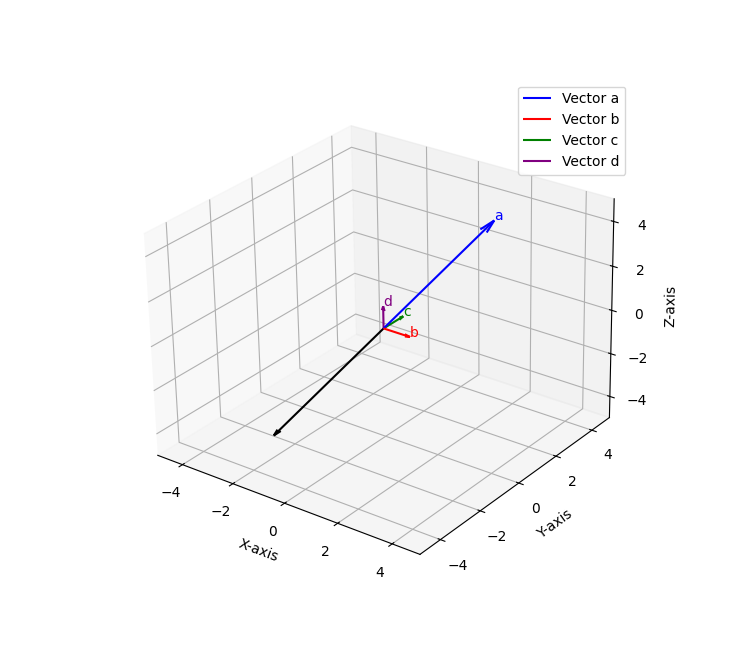
\includegraphics[width=0.8\columnwidth]{../figs/fig1.png}
\caption{}
\label{fig:1}
\end{figure}
\end{frame}

\begin{frame}{Plot by Python only}
\begin{figure}[H]
\centering
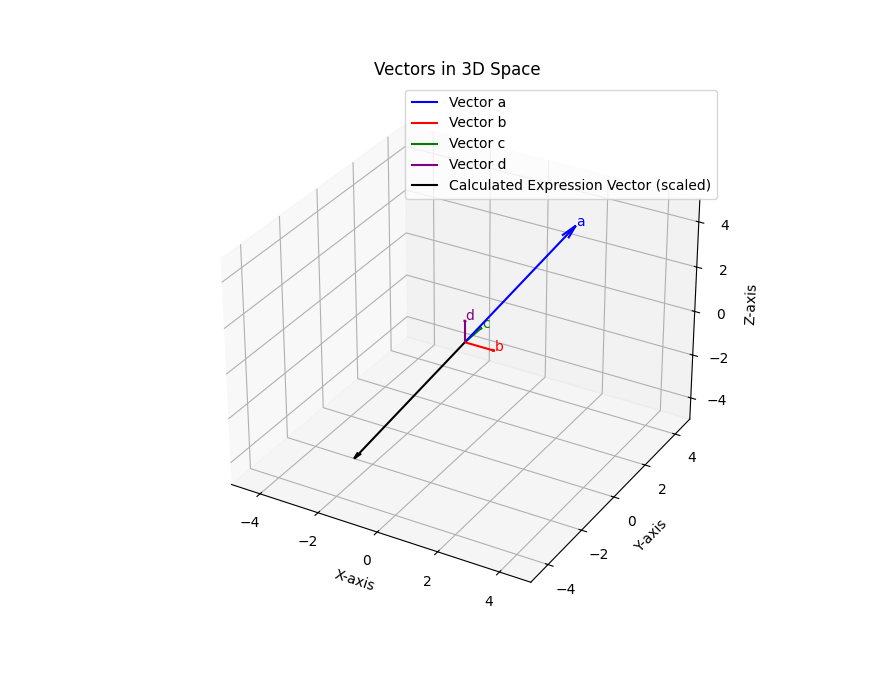
\includegraphics[width=0.8\columnwidth]{../figs/fig2.png}
\caption{}
\label{fig:2}
\end{figure}
\end{frame}

\end{document}
